\documentclass{article}
\usepackage{amsmath, amssymb, amsthm}
\newcommand\numberthis{\addtocounter{equation}{1}\tag{\theequation}}
\usepackage{tikz}

\title{Exercies of Chapter 9}
\author{Xiaoyu Chen}
\date{}

\begin{document}
\maketitle
\section{Exercise 9.4}
In Chapter 9, the jerrum book gives the general definition of the Dirichlet form:
\[\mathcal{E}_P(f, g) = -\mathbb{E}_\pi[fQg], \hspace{0.5cm} \mbox{where }Q = P - I\]
Show that
\[\frac{1}{2}\sum_{x, y} \pi(x)P(x,y)(f(y) - f(x))(g(y) - g(x))\]
is equal to $\mathcal{E}_P(f, g)$ when either $f = g$ or $P$ is time reversible,
and provide a counterexample to the equivalence in general.
\subsection{Solution}
Lets consider the general case first:
\begin{align*}
  \mathcal{E}_P(f, g) &= -\mathbb{E}_\pi [fQg] \\
  &= -\sum_{x\in\Omega} \pi(x)f(x)[Qg](x) \\
  &= -\sum_{x\in\Omega} \pi(x)f(x)\sum_{y\in\Omega}Q(x, y)g(y) \\
  &= \sum_{x, y\in\Omega} \pi(x) f(x)(I(x, y) - P(x, y)) g(y) \\
  &= \sum_{x\in\Omega} \pi(x) f(x)g(x) - \sum_{x, y\in\Omega} \pi(x)P(x, y)f(x)g(y) \\
  &= \frac{1}{2}\sum_{x\in\Omega} \pi(x)f(x)g(x) + \frac{1}{2}\sum_{y\in\Omega} \pi(y)f(y)g(y) - \sum_{x,y\in\Omega} \pi(x)P(x, y) f(x)g(y)\\
  &= \frac{1}{2}\sum_{x\in\Omega}\pi(x)f(x)f(x)\sum_{y\in\Omega}P(x,y) + \frac{1}{2}\sum_{x, y\Omega} \pi(x)P(x,y)f(y)g(y) - \sum_{x,y\in\Omega}\pi(x)P(x,y)f(x)g(y) \\
  &= \frac{1}{2}\sum_{x,y\in\Omega}\pi(x)P(x,y)f(x)f(x) + \frac{1}{2}\sum_{x, y\Omega} \pi(x)P(x,y)f(y)g(y) - \sum_{x,y\in\Omega}\pi(x)P(x,y)f(x)g(y) \numberthis \label{eqn:1}
\end{align*}
At the same time, we have
\begin{align*}
  \frac{1}{2}\sum_{x,y\Omega}\pi(x)&P(x,y)(f(y) - f(x))(g(y) - g(x)) \\
  &= \frac{1}{2}\sum_{x,y} \pi(x)P(x, y) (f(y)g(y) + f(x)g(x) - f(x)g(y) - f(y)g(x)) \numberthis \label{eqn:2}
\end{align*}
By comparing Equation \eqref{eqn:1} and \eqref{eqn:2}, we could know that
\[\mathcal{E}_P(f, g) = \frac{1}{2}\sum_{x,y}\pi(x)P(x,y)(f(y) - f(x))(g(y) - g(x))\]
iff
\[\sum_{x,y}\pi(x)P(x,y)f(x)g(y) = \sum_{x,y} \pi(x)P(x,y) f(y)g(x) \numberthis \label{eqn:3}\]
So, when $f = g$, its easy to verify that Equation \eqref{eqn:3} is true.
And when $P$ is time reversible, we have
\[\pi(x)P(x, y) = \pi(y)P(y,x)\]
, which means:
\begin{align*}
    \sum_{x,y} \pi(x)P(x,y)f(x)g(y) &= \sum_{x,y} \pi(y)P(y,x)f(x)g(y) \\
  &= \sum_{x,y} \pi(x)P(x,y)f(y)g(x), \hspace{0.5cm} \mbox{by swapping $x$ and $y$}
\end{align*}
To give a counterexample, we only need to give a MC and give two function $g, f$ where:
\[\sum_{x\not=y} \pi(x)P(x,y)f(x)g(y) \not= \sum_{x\not=y} \pi(x)P(x,y)f(y)g(x)\]

Consider a MC like this:
\begin{center}
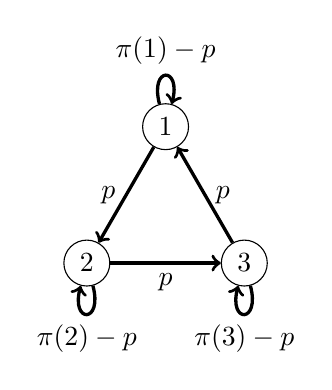
\begin{tikzpicture}
  [point/.style={shape=circle, draw=black, inner sep=3pt, minimum size=5pt}]
  \node (1) [point] at (0, 0) {$1$};
  \node (2) [point] at (-1, -1.732) {$2$};
  \node (3) [point] at (1, -1.732) {$3$};
  \draw [->, very thick] (1) to node [left] {$p$} (2);
  \draw [->, very thick] (2) to node [below] {$p$} (3);
  \draw [->, very thick] (3) to node [right] {$p$} (1);
  \draw [->, very thick, loop above] (1) to node [above] {$\pi(1) - p$} (1);
  \draw [->, very thick, loop below] (2) to node [below] {$\pi(2) - p$} (2);
  \draw [->, very thick, loop below] (3) to node [below] {$\pi(3) - p$} (3);
\end{tikzpicture}
\end{center}
The \textbf{edge measure} (i.e. $\pi(x)P(x,y)$) of each edge is marked in the figure.
It is clear that this MC is not time reversible.
In this MC, we have
\begin{align}
  \sum_{x\not=y}\pi(x)P(x,y)f(x)g(y) &= p(f(1)g(2) + f(2)g(3) + f(3)g(1))  \label{eqn:left} \\
  \sum_{x\not=y}\pi(x)P(x,y)f(y)g(x) &= p(f(2)g(1) + f(3)g(2) + f(1)g(3))  \label{eqn:right}
\end{align}
To give a counterexample, we only need to make $\eqref{eqn:left} - \eqref{eqn:right} \not= 0$, which means
\begin{align}
f(1)[g(2) - g(3)] + f(2)[g(3) - g(1)] + f(3)[g(1) - g(2)] \not= 0 \label{eqn:fg}
\end{align}
Consider an assignment for $f$ where $f = [1, 2, 1]$, and the Equation \eqref{eqn:fg} will become:
\[g(3) - g(1)\]
To make $g(3) - g(1)\not=0$, we could set $g$ to $[0, 0, 1]$.

\section{Exercise 9.8}
Verify identity (9.12).
\subsection{Solution}
First, we could notice that
\begin{align*}
  \pi(\Omega_0)\mathcal{L}_{\pi_0}(f) &+ \pi(\Omega_1)\mathcal{L}_{\pi_1} \\
  &= \mathbb{E}_\pi [f^2\ln f^2] - \sum_{b} \pi(\Omega_b)\mathbb{E}_{\pi_b}[f^2\ln (\mathbb{E}_{\pi_b}f^2)] \numberthis \label{eqn:12p}
\end{align*}
then we have
\begin{align*}
  \mathcal{L}_\pi(f) - \eqref{eqn:12p} &=  \sum_{b} \pi(\Omega_b)\mathbb{E}_{\pi_b}[f^2\ln (\mathbb{E}_{\pi_b}f^2)] - \mathbb{E}_\pi [f^2\ln(\mathbb{E}_\pi f^2)]  \\
                                       &= \sum_{b} \pi(\Omega_b)\mathbb{E}_{\pi_b}[f^2\ln (\mathbb{E}_{\pi_b}f^2)] - \sum_b \pi(\Omega)_b \mathbb{E}_{\pi_b} [f^2\ln(\mathbb{E}_\pi f^2)]  \\
                                       &= \sum_b \pi(\Omega_b) \mathbb{E}_{\pi_b} [f^2\ln(\mathbb{E}_{\pi_b}f^2) - f^2\ln(\mathbb{E}_{\pi}f^2)] \\
  &= \mathcal{L}_\pi(\bar{f})
\end{align*}

\section{Exercise 9.14}
By exhibiting a suitable graph, show that the bound in Example 9.13 is of correct order of magnitude, at least in some circumstances.
\subsection{Solution}
\begin{center}
  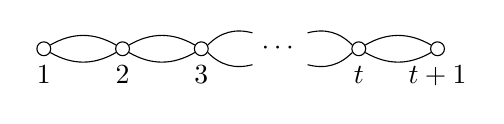
\begin{tikzpicture}
    [point/.style={shape=circle, draw=black, inner sep=0mm, minimum size=5pt}]
    \node (1) [point, label = below:$1$] at (0, 0) {};
    \node (2) [point, label = below:$2$] at (1, 0) {};
    \node (3) [point, label = below:$3$] at (2, 0) {};
    \node (4) at (3, 0) {$\cdots$};
    \node (5) [point, label = below:$t$] at (4, 0) {};
    \node (6) [point, label = below:$t+1$] at (5, 0) {};
    \draw [bend left = 30] (1) to (2);
    \draw [bend right = 30] (1) to (2);
    \draw [bend left = 30] (3) to (2);
    \draw [bend right = 30] (3) to (2);
    \draw [bend left = 30] (3) to (4);
    \draw [bend right = 30] (3) to (4);
    \draw [bend left = 30] (5) to (4);
    \draw [bend right = 30] (5) to (4);
    \draw [bend left = 30] (5) to (6);
    \draw [bend right = 30] (5) to (6);
  \end{tikzpicture}
\end{center}
In this graph, we have $n = t+1$ vertices with $m = 2t$ edges.
Any spanning tree of this graph should be a path that connect all the vertices.
And it is easy to note that the MC is now reduced to the random walk on hypercube $\{0, 1\}^t$ with $p = \frac{1}{t^2}$. Then by using the result of Exercise 8.14, we could find that the mixing time of this MC has a lower bould of $\Omega(t^2\log t)$ which is the same order of magnitude of $\Omega(mn\log n)$.

\section{Exercise 9.18}
Verify that $D(\sigma || \tau)$ is non-negative, and that $D(\sigma||\tau)=0$ implies $\sigma = \tau$.
\subsection{Solution}
\begin{align*}
  D(\sigma || \tau) &= \sum_{x\in\Omega} \sigma(x) \ln \frac{\sigma(x)}{\pi(x)} \\
  &= \sum_{x\in\Omega} \sigma(x) [- \ln \frac{\pi(x)}{\sigma(x)}] \\
  &= \mathbb{E}_{\sigma} [-\ln \frac{\pi(x)}{\sigma(x)}], \hspace{0.5cm} \mbox{by Jensen's Inequality} \\
  &\geq -\ln \mathbb{E}_\sigma [\frac{\pi(x)}{\sigma(x)}] \\
  &= -\ln [\sum_{x\in\Omega}\sigma(x) \frac{\pi(x)}{\sigma(x)}] \\
  &= -\ln 1 = 0
\end{align*}
The Jensen's Inequality achieves equality when all the possible parameter for $-\ln$ are the same (since $-\ln$ is non-linear). So we have
\[\frac{\pi(e_1)}{\sigma(e_1)} = \frac{\pi(e_2)}{\sigma(e_2)} =  \cdots =  \frac{\pi(e_n)}{\sigma(e_n)} = t\]
And by
\[\sum_{e\in\Omega} \pi(e) = t\sum_{e\in\Omega}\pi(e)\]
we know that $t = 1$, which means $\sigma = \pi$.
\end{document}

%%% Local Variables:
%%% mode: latex
%%% TeX-master: t
%%% End:
